\section{Présentation de l'entreprise}

\subsection{Fiche d'identite}
Sopra Steria est une entreprise caractérisée par :\newline
\begin{itemize}
	\item \textbf{Raison sociale :} Sopra Steria Group
\item  \textbf{Situation géographique :} 
\begin{itemize}
\item Siège social : Sopra Steria Group, 3 rue du pré Faucon, petite avenue des glaisins, 74940 Annecy, France 
\item Entreprise d'accueil : Sopra Steria Tourcoing, 41 ter avenue de la Marne, 59200 Tourcoing, France
\end{itemize}
\item  \textbf{Domaines d'activités :}
\begin{itemize}
	\item Consulting,
	\item intégration de systèmes,
	\item informatique scientifique, technique et embarquée,
	\item application management,
	\item testing,
	\item PLM-CIMPA
	\item infrastructure management
	\item business process services
	\item software
\end{itemize}
\item \textbf{Principaux clients :} Airbus, La Banque Postale, Cabinet Office, Ministère de la Défense,
EDF, Ministère des Finances, SNCF, EasyJet,...
\item \textbf{Principaux concurrents :} IBM, HP EDS, CSC, Accenture, CGI, Capgemini, Atos,
TCS, Cognizant, Wipro, Infosys
\item \textbf{Effectif :} 41661 salariés, 18649 en France fin 2017
\item \textbf{Résultat de l'année 2017 :} 3,845 milliards d'euros, dont 1,591 milliards d'euros en
France

\end{itemize}

\subsection{Historique}
\begin{itemize}
\item \textbf{1968-1985 : UNE RÉPONSE AUX BESOINS D'INFORMATISATION DE
	LA SOCIÉTÉ } L'industrie des services informatiques, tout juste naissante, accompagne la
modernisation de la Société. Sopra et Steria se fixent des objectifs de croissance ambitieux
pour atteindre une taille critique au plus vite et répondre aux besoins des grands comptes
par des produits et services innovants. Sopra investit dans le développement de logiciels et
multiplie les marchés verticaux. Parallèlement, Steria réalise de grandes signatures dans
la sphère publique.
\item \textbf{1985-2000 : LE TEMPS DE LA REFONDATION }Après deux décennies de dynamisme
exacerbé, le marché des services informatiques entame une phase de maturité
et affronte ses premières épreuves. En 1985, Sopra repense ses fondamentaux. Le modèle
combinant deux métiers complémentaires se dessine, la Société se recentre sur l'intégration
de systèmes et l'édition de logiciels. La performance économique est mise au coeur de la
stratégie pour assurer l'indépendance du Groupe dans la durée et préparer l'introduction
en Bourse, qui intervient en 1990. Steria réorganise également sa structure fonctionnelle. La rationalisation et l'industrialisation
des processus assurent à nouveau de beaux succès commerciaux. Les conditions
sont réunies pour permettre à la Société de planifier son introduction en Bourse en 1999. 
\item \textbf{2000-2014 : LA CONTRIBUTION A LA TRANSFORMATION NUMÉRIQUE
	DES CLIENTS }L'éclatement de la bulle Internet en 2001 accélère les mutations du
marché. Les clients recherchent des acteurs globaux, capables de les accompagner dans
la transformation de leurs métiers. Steria répond à ces enjeux par des acquisitions majeures
et structurantes. Le Groupe double de taille en intégrant les activités européennes
de Bull en 2001 et se renforce dans le conseil avec l'acquisition de l'allemand Mummert
Consulting en 2005. Xansa, Groupe Britannique, expert du BPO (Business Process Outsourcing),
entre dans le giron de Steria en 2007. La signature de l'un des plus gros contrats
de son histoire en 2013 avec le Gouvernement britannique renforce son ancrage dans le
secteur public. Sopra combine croissance interne et externe pour consolider son expansion
européenne et ses pôles de compétences, le conseil, l'intégration de systèmes et l'édition
de solutions. Axway, filiale née du regroupement des divisions d'infrastructure logicielle
du Groupe, est introduite en Bourse en 2011 pour poursuivre sa croissance de manière
autonome et partir à la conquête des États-Unis. Sopra est reconnu pour son expertise
dans les services financiers, ce qui conduit à la création de Sopra Banking Software en
2012. Les solutions dédiées aux Ressources Humaines sont regroupées en 2014 au sein de
la filiale Sopra HR Software.
\item \textbf{2014-2017 : UNE NOUVELLE DIMENSION UNE ACCENTUATION DE LA
	PERFORMANCE }Du fait des mutations induites par la transformation digitale, les
problématiques métiers montent en puissance au sein du marché des services numériques.
Dans ce contexte, le rapprochement amical de Sopra et Steria prend tout son sens et donne
naissance le 31 décembre 2014 à un nouveau leader européen de la transformation digitale,
Sopra Steria. La complémentarité des deux acteurs en matière de métiers, de verticaux
stratégiques et de géographies est idéale et les cultures d'entreprise sont proches. Dès les
premiers mois de 2015, le plan d'intégration construit conjointement par les équipes de
Sopra et de Steria est décliné avec succès dans les directions opérationnelles et fonctionnelles
du nouveau Groupe. Dans le même temps, le Projet Sopra Steria 2020 est lancé
pour améliorer la performance dans tous les domaines et augmenter la valeur ajoutée.
En s'appuyant sur une offre endto-end délivrée aux grands clients selon une approche
verticale, ce projet favorise les initiatives dans le domaine du Digital et met l'accent sur
le conseil et l'édition de solutions, par croissance interne et externe. En 2016, le Groupe
lance New Way, un programme sur 3 ans visant à fédérer l'ensemble des collaborateurs
autour d'une même culture et de fondamentaux partagés. Le plan d'actionnariat salarié
We Share associe plus étroitement encore les salariés au développement du Groupe. Avec
environ 8% du capital détenu par ses collaborateurs, Sopra Steria est la première entreprise
française de services du numérique en matière d'actionnariat salarié. En appui du
Projet Sopra Steria 2020, les investissements stratégiques dans les services, le conseil et
l'édition de solutions métiers se poursuivent. L'acquisition de CIMPA en octobre 2015
permet au Groupe d'intensifier sa présence sur le marché du PLM (Product Lifecycle
Management). Finalisé en janvier 2017, le rapprochement avec l'éditeur Cassiopae renforce
Sopra Banking Software dans les solutions de gestion des financements spécialisés.
Sopra Steria apporte une réponse globale aux enjeux de développement et de compétitivit
é des grandes entreprises et organisations. Combinant connaissance fine des métiers,
valeur ajoutée, innovation et performance des services délivrés, l'entreprise accompagne
ses clients dans cette transformation et les aide à faire le meilleur usage du numérique
\end{itemize}

\subsection{Implantation géographique}
Comme le montre la figure \ref{monde}, extraites extraites d'un document de référence de l'entreprise, Sopra
Steria est présent aussi bien en France qu'à l'étranger. Le Groupe fait également parti des 5
premiers acteurs européens et des 10 premiers opérant en Europe.\newline
\begin{figure}[!h]
%	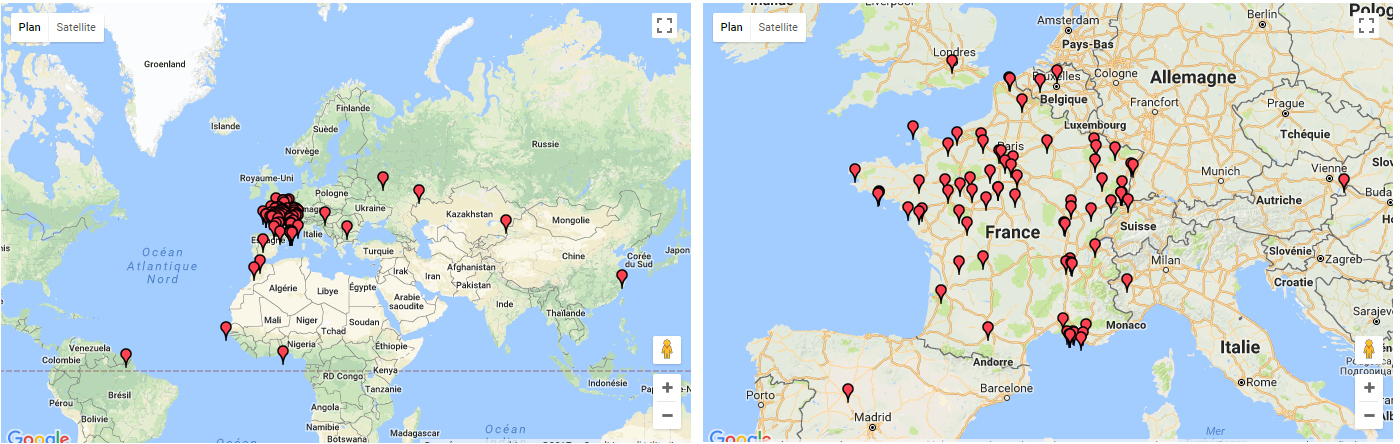
\includegraphics[width=\textwidth]{monde.png}
	\centering \caption{Cartes de l'implantation géographique de Clemessy.}
	\label{monde}
	\centering
\end{figure}
\subsection{Activités}
Les activités de Sopra Steria sont nombreuses. Parmi elles, on trouve le Consulting, l'Inté-
gration de systèmes, l'Informatique Scientifique, Technique et embarquée, l'Application Management,
le Testing, le PLM-CIMPA, l'Infrastructure Management, le BusinessProcess Services,
le Software
\subsection{Organisation}
\begin{figure}[!h]
%	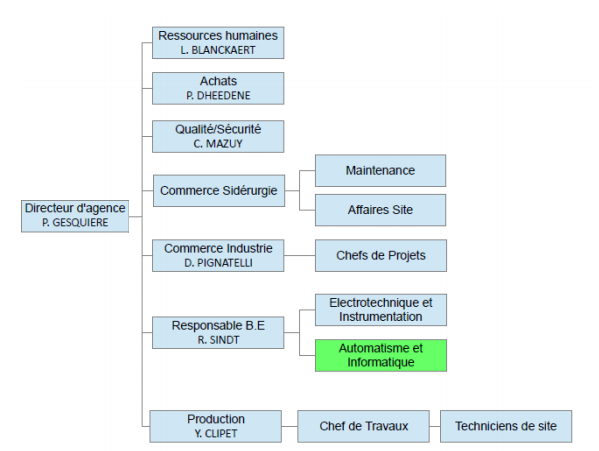
\includegraphics[scale=0.9]{organigramme.png}
	\centering \caption{Organisation hiérarchique de Sopra Steria Tourcoing.}
	\label{organigramme}
	\centering
\end{figure}
\subsection{Chiffres-clés}Comme indiqué sur le site de Sopra Steria, le Groupe emploie près de 42000 collaborateurs
en France et à l'international dans plus de 20 pays. C'est également 3,8 milliards d'euros de
chiffre d'affaires en 2017 dont 51\% sont effectués en France et 22\% au Royaume-Uni.
Les métiers sont à 60\% en Conseil et Intégration de Systèmes, 16\% en Solutions, 13\% en gestion
d'infrastructures informatique et 10\% de Business Process Services. Sopra Steria développe à
23\% dans le domaine des banques, à 22\% dans le secteur public, 18\% dans l'aérospatial, défense
et sécurité intérieure, 6\% dans les transports.
\subsection{Mon poste}
Dans l'entreprise, je travaillais à Tourcoing, au Centre de Service SNCF AURORE, pour le
projet HUBIC. J'avais pour chef de projet Damien LOHEZ, et sur le projet, j'étais accompagné
par un second développeur TIBCO, Youssef JOUHRI, le responsable d'application Nabil EL
MOUATS et la team leader, Asmaa ETTOUIMI. Ces dernières étant situées à Meudon-La-
Forêt. Je devais aider au développement du projet en TIBCO et également comprendre le
fonctionnement de plusieurs autres projets au sein du CDS.